\documentclass[11pt,a4paper]{article}
\usepackage[UTF8,fontset=none]{ctex}
\setCJKmainfont{Noto Serif CJK SC}[BoldFont={Noto Sans CJK SC Bold}]
\setCJKsansfont{Noto Sans CJK SC}
\setCJKmonofont{Noto Sans Mono CJK SC}
\setmainfont{Liberation Serif}
\setsansfont{Liberation Sans}
\setmonofont{Liberation Mono}
\usepackage{amsmath,amssymb,graphicx,booktabs,array,geometry,caption,hyperref,flafter}
\geometry{left=24mm,right=24mm,top=24mm,bottom=25mm}
\hypersetup{colorlinks=true,linkcolor=black,citecolor=black,urlcolor=blue,
 pdftitle={覆盖约束下的语义条件主动观察与设施三维建档},pdfauthor={李兆宇}}
\captionsetup{font=small,labelfont=bf,labelsep=quad}
\setlength{\parskip}{3pt}
\setlength{\emergencystretch}{2em}
\linespread{1.16}
\newcommand{\J}{J_{5}}
\newcommand{\C}{C_{\mathrm{map}}}
\newcommand{\F}{F_{1,5\mathrm{cm}}}
\newcommand{\figpath}{docs/thesis/figures/v38/}
\title{\textbf{覆盖约束下的语义条件主动观察与设施三维建档}\\[5pt]
\large 保留ANS层次与四模块接口的CPU机制验证}
\author{李兆宇}
\date{2026年9月20日研究论文修订稿}
\begin{document}
\maketitle
\begin{abstract}
二维区域已被观察不代表其中设施已经得到完整三维建档。本文研究有限运动预算下，设施类别知识能否在几何证据尚不充分时提示有效观察方向。保留ANS全局与局部层次及四模块接口，构建语义条件构型信念、预算约束的滚动观察规划和实测几何反馈；预测模板只参与规划，三维模型由已执行深度观测独立融合。以二维覆盖率与设施表面F1的乘积为主指标，同时报告覆盖、精确率、完整率与任务资格。在控制器冻结的两个父布局、每布局两个构型、共八条G/S确认任务中，语义方法相对具备主动补看能力的几何对照，平均联合终点由0.7026提高至0.7459，相对提高6.16\%；两种零增量构型完整保留，全部任务满足预算、覆盖和安全返航要求。开发实验中的类别置换与后验干预进一步支持语义选向及错误先验纠正机制；独立的早期学习型收益头实验提供条件预测的补充证据，但覆盖压力层无语义增益。结果支持公开设施先验下的受控虚拟建档方案，并界定其对观察需求、预算阶段和先验可靠性的依赖。自然语义识别、原神经ANS和外部完整系统比较仍需另行验证。
\end{abstract}
\noindent\textbf{关键词：}主动观察；语义条件规划；设施建档；二维覆盖；表面重建；层次规划

\section{引言}
工业设施巡查、机房资产建档与实验室设备数字化，既需要了解机器人可达区域，也需要记录设施的外表面、凹入结构和被遮挡的服务侧。携带单线激光雷达与窄视场深度相机的地面机器人，可能已经完成通道覆盖，却只获得设施正面的片段。此时继续扩大二维已知区域的收益有限，而从合适方向获取少量新观测可能改善三维档案。任务的实际困难在于：机器人应在到达观察位置之前判断这次移动是否值得。

语义类别可以携带结构规律。例如，类别与服务侧、开口或遮挡面的位置相关时，类别观测可以帮助选择观察方向。然而，“复杂设施值得多看”并不构成充分的规划策略。重复观察同一可见面可能不增加有效信息；错误类别还可能把有限预算引向错误方向。几何方法同样可以依据已观测缺口、可见性与不确定性主动补看。因此，语义的价值必须体现为共同几何信息之外的决策增量，并最终落实到实测重建质量。

本文采用机制隔离的研究路线。首先保留Active Neural SLAM（ANS）的全局目标选择与局部执行层次\cite{chaplot2020}，明确开放词汇语义密度场（OV-SDF）、语义拓扑图层次规划（STGHP）、不确定性感知可达性预测（RPN-UQ）和信息增益覆盖奖励（IGCR）的接口职责。随后，在CPU可复核原型中检验“类别线索—构型信念—观察决策—重建质量”的链条。这里的模块名称是架构接口约束；当前确认实验运行确定性机制实现，不把接口调用视为相应神经网络已经得到验证。

研究围绕三个问题展开。H1：当已观测几何不能区分有效观察方向时，类别条件信息是否改变动作？H2：在同一传感、建图后端、动作预算和任务资格要求下，该信息能否提高联合建档结果？H3：实际观测能否修正误导先验，并减少其造成的质量损失？H1/H2通过冻结控制器的配对确认检验；H3由开发期错误类别政策比较及同状态后验干预提供有限证据，不与确认结果合并扩大样本量。

本文的工作包括三个相互关联的部分：构建具有明确输入权限的语义条件主动观察机制；以几何控制、类别置换和反馈政策对照检验作用来源；整理具有冻结协议、完整负例、独立回放及逐项指标的证据链。贡献的范围是设施建档中的条件观察价值与可复核实现，尚不包括大规模未知场景探索、位姿估计改进或相对主流完整系统的性能领先。

\section{相关工作与研究定位}
\subsection{层次化几何探索}
ANS把学习式建图、全局策略与局部策略结合分析式规划，提供模块化探索组织方式\cite{chaplot2020}。TARE通过局部密集与全局粗粒度表示安排探索路线；其后续工作进一步研究表示粒度与复杂环境探索效率\cite{cao2021tare,cao2023granularity}。FUEL维护增量前沿并进行层次规划，FALCON以覆盖路径引导前沿访问顺序\cite{zhou2021fuel,zhang2025falcon}。这些方法说明，主动获取几何信息和安排观察顺序本身已是强基线能力。本文的内部几何对照保留主动获取构型信息、覆盖代理、预算规划和返航能力，不能等同于只访问最近前沿的弱对照。

\subsection{语义巡检、预测与任务相关建图}
SWAP已将语义目标检查、未充分观测区域和观察质量条件纳入探索规划\cite{dharmadhikari2023swap}。SPP进一步利用语义场景图中的重复结构预测尚未观察的目标，并处理预测与实际环境不一致的情况\cite{dharmadhikari2025spp}。因此，语义引导补看及预测后纠错并非本文首次提出；当前双构型先验也不等价于SPP所需的重复子图。

ActiveSGM在语义与几何不确定性作用下执行主动建图，采用3D Gaussian Splatting表示\cite{chen2025activesgm}。VISTA把开放词汇任务相关性、视向覆盖和在线语义高斯地图结合\cite{nagami2026vista}。这些方法与本文共享“任务信息影响观察分配”的问题，但原任务、表征、前端和计算资源不同。直接复制它们原论文的分数与本项目TSDF结果比较，无法区分规划、感知和重建后端的贡献。

\subsection{本文的具体检验对象}
本文关注一个有限但可辨识的条件：已发现设施的当前几何历史不足以区分互补观察方向，类别线索却与公开的结构知识相关。共同深度融合使用Open3D的CPU TSDF实现\cite{zhou2018open3d}；所有方法的实测模型均由实际取得的深度构建。类别可以改变规划中的构型权重，不能改变评价器中的类别权重，也不能把假设表面直接加入模型。这样的实验可回答语义信息如何产生收益，但尚不足以排除所有其他语义规划机制都能获得相同收益。外部比较应作为单独实验完成，见第\ref{sec:external}节。

\section{任务定义与评价原则}
\subsection{任务、信息与约束}
设机器人状态为离散姿态$s_t=(x_t,y_t,\theta_t)$，动作历史为$a_{0:t-1}$，观测历史为$\mathcal H_t=(o_{0:t},a_{0:t-1})$。观测包含已执行动作后取得的RGB-D、平面扫描和位姿。对设施真实构型$h\in\{0,1\}$，规划器维护权重$p_t(h)$；它可以读取两种公开模板、共同安全图及设施坐标系，却不知道哪个模板是真实构型。评价器独占真实构型和参考表面。

目标是在总动作预算$B$内完成观察并返回起点。前进1 m与转向90度各计一次，避免把原地转向或补拍当作免费观测。当前确认协议固定$B=42$，前18个动作是共同观测前缀，余下最多24个动作由策略滚动选择。该协议检验完成共同前缀后的建档规划，不代表从动作0自主完成未知场地探索。

任务资格独立要求：覆盖率不低于80\%、无碰撞、预算内完成并精确返回起点及初始朝向。原始质量指标与资格同时报告，质量提高不能抵消未返航或覆盖不合格。公开安全图提供可行运动边；这属于带场地先验的建档设置，不能用执行成功推断未知环境中的概率安全保证。

\subsection{二维覆盖与三维表面质量}
在固定公共域内，以0.2 m栅格和0.2 m机器人半径确定从起点可达的安全格集合$\mathcal R$。令$m_T(c)=-1$表示未知，则
\begin{equation}
\C(T)=\frac{\left|\{c\in\mathcal R:m_T(c)\ne-1\}\right|}{|\mathcal R|}.
\label{eq:coverage}
\end{equation}
已判为占据的格子也计为已知。因此该量衡量观察覆盖，不衡量占据分类准确率；实际控制器不依靠当前实测占据栅格重新建立安全图。两个父布局P00/P01的分母固定为588/668，不能随方法路径改变。

设预测网格的面积均匀采样点集为$\widehat{\mathcal S}$，参考外竖面采样点集为$\mathcal S_v$，完整参考表面为$\mathcal S$。距离阈值$\tau$下
\begin{align}
P_\tau&=\frac{1}{|\widehat{\mathcal S}|}\sum_{q\in\widehat{\mathcal S}}
\mathbf1[d(q,\mathcal S)\le\tau],\\
R_\tau&=\frac{1}{|\mathcal S_v|}\sum_{q\in\mathcal S_v}
\mathbf1[d(q,\widehat{\mathcal S}_{\rm mesh})\le\tau],\qquad
F_{1,\tau}=\frac{2P_\tau R_\tau}{P_\tau+R_\tau}.
\label{eq:f1}
\end{align}
第一式距离实际查询完整参考网格，第二式查询预测网格，符号中的点集只定义采样分布。预测先按两构型共同AABB外扩0.20 m裁剪，再去除已知地面附近的近水平片段；没有补洞、配准或向真值吸附。每方向32768个固定种子采样点。ROI外错误不计入精确率，参考召回仅覆盖全部外竖面，因此这不是全场景三维精度。该不对称定义和裁剪规则对所有方法一致。

主指标为
\begin{equation}
\J(T)=\C(T)\F(T),\qquad \tau=0.05\ \mathrm m,
\label{eq:joint}
\end{equation}
并报告2 cm、10 cm阈值敏感性。当$P_\tau+R_\tau=0$时令$F_{1,\tau}=0$；空预测的$P,R,F_1,J$均为0，距离误差为空值而非零误差。乘积是一种透明的任务效用，不单凭此形式宣称新理论；必须分解覆盖、精确率和完整率才能解释收益。在当前配对结果中覆盖相同，$J$提高来自表面F1改善，不能写成覆盖与定位精度同时提高。

\subsection{早期证据采用的另一指标}
早期学习型实验的目标是共同前缀后的面积联合增量
\begin{equation}
\Delta J_A=A_{2D}(T)F_{1,5\mathrm{cm}}^{\rm global}(T)
-A_{2D}(t_0)F_{1,5\mathrm{cm}}^{\rm global}(t_0).
\label{eq:legacy}
\end{equation}
其单位为m$^2$，三维参考范围也不同于式\eqref{eq:f1}。它用于检验接近完成覆盖时的补看预算分配，与终点归一化$J_5$分别作表和统计，不拼接为算法逐轮提升曲线。对任一队列，相对效应均计算为$(\overline y_S-\overline y_G)/\overline y_G$，同时提供绝对差。

\section{语义条件层次观察方法}
\subsection{四模块实现与信息隔离}
图\ref{fig:architecture}给出最终在线CPU实现。OV-SDF接口收集观测与地图摘要并形成类别条件先验；STGHP选择姿态子目标；RPN-UQ执行图边及返航预算检查；IGCR以实测残差更新构型权重。系统保留ANS全局—局部结构，但没有运行原ANS的神经SLAM、全局PPO与局部模仿学习网络。表\ref{tab:modules}区分已执行机制与尚未验证的原设计能力。

\begin{figure}[tb]
\centering\includegraphics[width=\linewidth]{\figpath fig01_architecture.pdf}
\caption{实际CPU闭环与四模块接口。语义先验和几何反馈影响全局选向，局部守卫约束动作和返航成本；共享TSDF仅融合已执行深度。虚线下方为封存后的独立评价。公开模板预测参与规划，不作为新增真实观测或补入预测网格。}
\label{fig:architecture}
\end{figure}

\begin{table}[tb]
\centering\small
\caption{架构名称与当前证据对应。四接口执行不等于四个神经模块均具有独立消融收益。}
\label{tab:modules}
\begin{tabular}{p{.13\linewidth}p{.39\linewidth}p{.38\linewidth}}
\toprule
接口 & 在线实现 & 尚未由本批验证的能力\\\midrule
OV-SDF & 人工RGB类别账本、地图摘要、类型条件权重 & 自然开放词汇检测、语义场学习、多实例关联\\
STGHP & 公开姿态图上的有限预算滚动选向 & 未知场景在线拓扑学习、大规模效率\\
RPN-UQ & 边合法性及确定性返航预算检查 & 学习式到达概率、不确定性校准\\
IGCR & 首次姿态几何残差更新及冲突处理 & 真实重建奖励在线学习、普遍正反馈收益\\\bottomrule
\end{tabular}
\end{table}

控制器接收去除构型身份的观测记录，而不接收世界实例、隐藏构型ID或评价真值。候选模板与安全图是双方共享的规划知识。实际深度与扫描来自已付费动作后的传感包；规划时对公开模板的射线和曝光预测是先验计算，不得查询未选择动作的实际传感结果。每个已执行观测只融合一次，实际融合中的语义标签数组恒为零，从而把语义影响限制在观察选择链条。

\subsection{OV-SDF：类别条件权重与保守更新}
记几何和语义的对数权重分别为$L_t^g,L_t^s$，取
\begin{equation}
p_t(h=0)=\sigma(L_t^g+L_t^s),\quad p_t(h=1)=1-p_t(h=0).
\label{eq:belief}
\end{equation}
这里是鲁棒伪似然下的构型权重，不声称其数值是经过校准的真实概率。类别A/B与设施局部负/正$u$侧相关，这一类型—结构关系是公开人工知识；颜色本身不编码运动方向。

RGB中单帧至少16个同类标记像素、且没有另一颜色混入时，登记该类别支持。相同类别在两个不同XY位置得到支持后，一次性令$L^s=\pm\log(0.9/0.1)$；后续重复帧不再连乘置信。若出现冲突类别，清零类别先验。当前账本针对单设施，0.9为采集前固定值，未使用自然图像校准。G控制条件屏蔽类别信息并保持$L^s=0$，其几何更新和其他规划能力完整保留。

\subsection{IGCR：由实测残差修正结构假设}
两模板预测不同时，实测深度提供区分构型的证据。对模板$h$定义参考视差域损失
\begin{equation}
e_h^d=\frac{1}{N_d}\sum_i
\min\!\left\{\frac12\left(\frac{57.6/z_i-57.6/\widehat z_{h,i}}{0.25}\right)^2,\,12.5\right\}.
\label{eq:residual}
\end{equation}
其中仅使用有效实测深度，模板无返回时损失为12.5。实测零深度不被当成“存在隐藏表面”的证据。至少8个有效区分像素才使用深度模态；扫描至少3束有效区分射线，以0.02 m作为残差归一化尺度并采用相同截断损失。

将有效模态的$e_1-e_0$取平均并截断至$[-6,6]$，作为该姿态的几何增量；累计$L^g$截断至$[-24,24]$。只在每个精确$(x,y,\theta)$的首次观测累计后验。重复姿态的新深度仍可进入TSDF，但不会反复抬高构型置信。这种区分使几何证据足够时可以压过错误的0.9类别先验，同时降低相关观测重复计数的问题。

\subsection{STGHP：预测观察价值与预算规划}
对公开模板$h$，历史姿态的理想曝光掩码取集合并。每个设施的潜在已曝光竖面面积除以全部外竖面面积，设施间等权，得到$\widetilde F_h$；公开地面中心的理想曝光比例为$\widetilde C_h$。终端规划代理为
\begin{equation}
\widetilde J_h=\widetilde C_h\widetilde F_h.
\label{eq:proxy}
\end{equation}
$\widetilde F$是预测表面积比例，既非实测F1也非补全出的实际模型。集合并使已曝光区域不因重复停留而重复获得同等收益；观测价值由新增有效曝光及构型信息共同决定。

有限动态规划在剩余动作数内最大化后验加权的终端代理，并预估一次未来诊断事件的价值。若公开无噪声模板在某未访问节点产生足够不同的观测，且双向伪似然分别越过$\pm\log99$，规划器假设该节点提供正确率0.99的二元信息通道。令$z$为预测诊断输出，$\Pi$为图上策略，则其结构可表示为
\begin{equation}
\Pi_t^*=\arg\max_{\Pi\in\mathcal P(B-t)}
\mathbb E_{h\sim p_t,\,z\sim\widetilde p(z\mid h,\Pi)}
[\widetilde J_h(\Pi,z)] .
\label{eq:planning}
\end{equation}
实现中每次滚动前瞻最多展开一个诊断事件，并非完整POMDP最优求解。预测分支只改变规划值，动作执行后仍按实际残差更新，不直接写入0.99。G同样可以选择诊断视点；语义降低的是在初期选错方向或先探查再改向的预算代价。

\subsection{RPN-UQ：可行性与执行}
对下一姿态$s'$，局部守卫要求动作属于公开图边，且
\begin{equation}
1+d_{\mathrm{return}}(s')\le B-t.
\end{equation}
停止必须位于起点，且两个模板的理想覆盖代理均不低于80\%。每次规划最多150万缓存状态、20 s；同分按冻结图边顺序和$10^{-12}$容差选择。该守卫是确定性预算约束，不能等同于概率可达性模型。

每一循环依次完成：保存当前传感包并融合共同地图；更新类别账本及首次姿态的几何权重；累并两个模板的曝光集合；执行共同前缀或求下一姿态；核验图边与返航预算后执行。达到停止条件后封存动作、观测、网格和后验历史，再调用独立评价器。此顺序保证评价质量不反馈给当次规划。

\section{实验设计与可复现性}
\subsection{机制导向场景与证据分层}
场景设计刻意包含遮挡与互补观察：相同初始几何可以对应不同设施构型，类别线索先于区分几何出现；有限剩余预算使访问顺序可能影响最终质量。这对应有目录或设施知识的主动建档，而非任意室内探索。按机制设计场景有助于识别因果链，但也限制总体外推，故必须保留语义不改变最优动作的构型和覆盖压力反例。

表\ref{tab:cohorts}列出本文使用的证据队列。最终在线开发队列V35使用一个父布局P00、两个构型和四种条件；V36冻结相同控制器，在两个父布局和预定留出深度噪声种子上仅比较G/S。P01此前已有理想几何与像素筛查信息，因此不能称完全未见布局。早期学习型队列V11.1拥有独立冻结上下文，但其模型、目标与场景族均不同，只提供补充证据。

\begin{table}[tb]
\centering\small
\caption{证据队列、真正运行数量与统计单位。独立回放检验复现，不增加独立样本量。}
\label{tab:cohorts}
\begin{tabular}{p{.24\linewidth}rrp{.37\linewidth}}
\toprule
队列 & 主轨迹 & 回放 & 单位与用途\\\midrule
V35在线开发 & 8 & 8 & 1父布局$\times$2构型$\times$4条件；机制开发\\
V36在线确认 & 8 & 8 & 2父布局$\times$2构型$\times$G/S；描述性确认\\
V11.1学习型开发 & 56 & 56 & 4个已见父上下文；训练后闭环开发\\
V11.1学习型确认 & 96 & 96 & 8父上下文$\times$2布局$\times$6条件；组级推断\\
V11.1覆盖压力 & 40 & 40 & 4父上下文$\times$2布局$\times$5条件；边界检验\\\bottomrule
\end{tabular}
\end{table}

\subsection{共享传感、融合与噪声}
在线队列使用96$\times$72深度相机，焦距48 px，安装高度0.9 m、欧氏量程4 m；单线扫描高0.25 m，360度共180束，量程8 m。位姿完全准确，扫描未附加随机噪声。深度首次命中值$z$转入参考视差域，加入$\epsilon\sim\mathcal N(0,0.25^2)$ px后恢复
\begin{equation}
z'=\frac{57.6}{57.6/z+\epsilon}.
\end{equation}
57.6来自参考焦距480 px与0.12 m基线，参考焦距与成像内参48 px不同。该模型用于数值噪声敏感性检验，没有标定为实验室ZED的真实误差模型。随机源由父布局、已付费步和固定种子确定，不以类别决定噪声。V35/V36分别使用1901/350918。

共享CPU TSDF体素为4 cm、截断为12 cm，所有条件一致。距离测量使用固定采样种子340918/340919。5 cm是主阈值，2 cm低于体素尺寸，作为严格敏感性结果解释；不能只报告最有利阈值。所有阈值及表面距离分布保留在原始结果，图表从已保存数值生成，不重新运行模拟或重算重建质量。

\subsection{对照与干预}
G为主动几何：类别先验均匀，其余构型模板、残差更新、未来诊断、候选池与预算规划与S相同。S使用正确类别解释；X将类别解释交换，用于检验类型—结构关系是否重要；Xnf在X上同时关闭实测几何后验更新与规划中的未来纠错。X与Xnf比较的是整套纠错政策，不能解释为单独删去一个反馈函数的纯单因素消融。

V35另外保存两次预定同状态后验干预：固定姿态、曝光状态及共同历史，只改变用于决策的后验，检查所选动作是否改变。这提供反馈影响动作的证据，但没有执行新的反事实轨迹，因此不能为该干预单独赋予终点质量收益。V36只运行G/S，没有重新确认X/Xnf。RPN-UQ和STGHP的单独模块必要性也未在最终队列消融。

\subsection{统计、冻结与失败保留}
V35/V36的父布局为目的性构造，分别只有一个和两个；报告逐构型配对差与父布局等权均值，不以动作帧、表面点、阈值或回放作为独立样本计算显著性。V11.1确认则以8个父上下文为组，每组先平均两种类别布局，再使用已有的组级bootstrap区间及单侧符号检验；bootstrap为20000次整组重采样、种子11102，报告95\%百分位区间。后者仅适用于冻结人工机制族，不迁移至V36。

源码、配置、种子、测量定义和终端结果均有SHA清单；传感包、动作、后验与网格封存后进行独立复核。V36八条主轨迹及八条独立在线回放一致，另有只读验证器核验八任务共344份保存观测。开发失败和准备阶段结构门失败均保留。论文整理不新增物理回合，也不把重新绘图计为额外实验；逐项来源见附录\ref{app:evidence}。

\section{结果}
\subsection{冻结在线方案的联合建档效果}
表\ref{tab:confirmation}给出V36全部八个终点及指标分解。在P00上，G/S平均$J_5$为0.722452/0.766328，绝对差0.043876，相对差6.0732\%；P01为0.682699/0.725433，绝对差0.042734，相对差6.2596\%。两个父布局等权汇总为0.702576/0.745881，绝对提高0.043305，相对提高6.1638\%。该百分比是归一化联合分数的均值之比。

\begin{table}[tb]
\centering\small
\caption{V36冻结确认的完整终点结果。覆盖以百分数表示，其他指标取值0--1；所有行均42动作、零碰撞且精确返航。每父布局保留两个构型，未删去零收益对。}
\label{tab:confirmation}
\begin{tabular}{lllrrrrr}
\toprule
布局 & 构型 & 方法 & $C_{\mathrm{map}}$ (\%) & $P_5$ & $R_5$ & $F_{1,5}$ & $J_5$\\\midrule
P00 & $h_0$ & G & 95.75 & 0.8734 & 0.7491 & 0.8065 & 0.7722 \\
P00 & $h_0$ & S & 95.75 & 0.8734 & 0.7491 & 0.8065 & 0.7722 \\
P00 & $h_1$ & G & 95.75 & 0.8560 & 0.5958 & 0.7026 & 0.6727 \\
P00 & $h_1$ & S & 95.75 & 0.8781 & 0.7249 & 0.7942 & 0.7605 \\
P01 & $h_0$ & G & 94.76 & 0.8632 & 0.6909 & 0.7675 & 0.7273 \\
P01 & $h_0$ & S & 94.76 & 0.8632 & 0.6909 & 0.7675 & 0.7273 \\
P01 & $h_1$ & G & 94.76 & 0.8549 & 0.5555 & 0.6734 & 0.6381 \\
P01 & $h_1$ & S & 94.76 & 0.8633 & 0.6845 & 0.7636 & 0.7236 \\
\bottomrule
\end{tabular}

\end{table}

两个$h_0$构型中G/S轨迹和终点相同，说明类别并不必然产生收益。两个$h_1$构型在相同二维覆盖下获得较高的表面完整率：P00由0.5958提高至0.7249，P01由0.5555提高至0.6845；精确率分别由0.8560至0.8781、0.8549至0.8633。因而观察方向改变主要减少了未重建的外竖面，而不是借助降低覆盖要求获得高分。

\begin{figure}[tb]
\centering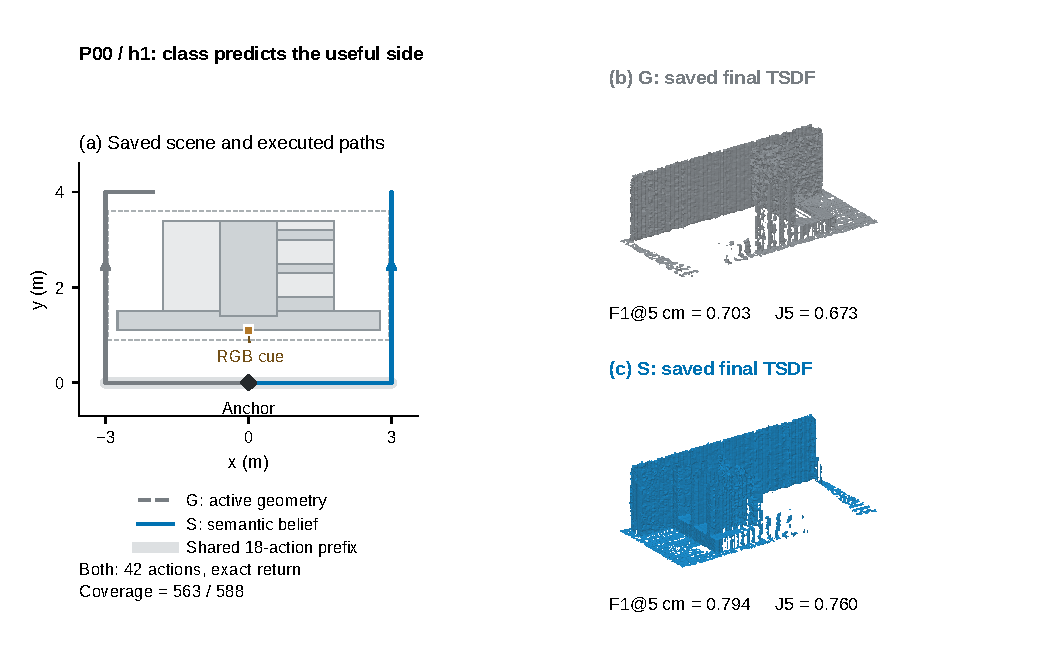
\includegraphics[width=\linewidth]{docs/thesis/figures/v38_qualitative/v38_saved_paths_and_tsdf.pdf}
\caption{P00/$h_1$的实际路径与保存终点重建。（a）离线场景几何和已执行G/S轨迹；（b、c）相同正交视角、坐标范围下的终点TSDF，绘制全部保存三角形，无简化、补洞或配准。颜色表示方法及显示光照，不是逐点误差。几何真值仅用于离线示意；这是正收益构型，$h_0$零增量见完整定量图。}
\label{fig:qualitative}
\end{figure}

\begin{figure}[tb]
\centering\includegraphics[width=\linewidth]{\figpath fig02_confirmation.pdf}
\caption{V36全部配对结果及阈值敏感性。（a）点为真实终点，文字为同构型S减G的绝对差；两个$h_0$的零差保留。（b）每父布局先平均两个构型，给出2/5/10 cm下的绝对差；5 cm为主阈值。两个父布局为目的性设计，图中不绘制总体置信区间，回放不作为新样本。}
\label{fig:confirmation}
\end{figure}

图\ref{fig:confirmation}显示三个预定距离阈值下父布局平均差均为正；总体相对差在2/5/10 cm分别为5.50\%、6.16\%、6.21\%。这是对当前表面阈值的稳定性检验，不等价于对不同场景族、多个随机种子或不同传感器的稳健性。各构型资格均通过，P00/P01覆盖率分别为95.7483\%/94.7605\%。

\subsection{收益是否由语义信息引起}
保存观测显示，在两个父布局的$h_1$中，第18个动作结束后G/S具有相同姿态、曝光掩码和非语义观测历史，尚未取得可区分真实构型的几何反馈。S的$h_1$权重为0.9，G为0.5；两者随后分别选择右转和左转，第19个动作开始出现实际分歧。该对照把语义作用定位到几何证据不足的决策窗口，而不是给几何组禁止补看的限制。

开发期类别干预与此解释一致。V35中S相对G的平均$J_5$提高6.5644\%，相对错误类别X提高14.7283\%（表\ref{tab:ablation}）。S/G的$h_0$仍完全相同，而类别交换使其下降。正确类别、无类别和错误类别之间的模式支持“类别与构型关系影响选向”的解释。它不能说明任意自然类别标签都会带来收益，也不能据此估计自然前端的识别准确率。

\begin{table}[tb]
\centering\small
\caption{V35开发期语义干预与纠错政策比较。各条件具有相同覆盖95.7483\%，均42动作并安全返航；均值对$h_0/h_1$等权。Xnf同时移除实际反馈与未来纠错预期。}
\label{tab:ablation}
\begin{tabular}{lrrrr}
\toprule
条件 & $J_5(h_0)$ & $J_5(h_1)$ & 平均$F_{1,5}$ & 平均$J_5$\\\midrule
G & 0.7723 & 0.6752 & 0.7559 & 0.7238 \\
S & 0.7723 & 0.7702 & 0.8055 & 0.7713 \\
X & 0.6693 & 0.6752 & 0.7021 & 0.6723 \\
Xnf & 0.6527 & 0.6574 & 0.6842 & 0.6551 \\
\bottomrule
\end{tabular}

\end{table}

\subsection{几何反馈的收益与局限}
错误类别下，V35的X/Xnf平均$J_5$为0.672254/0.655065，绝对提高0.017190，相对提高2.6241\%。后验时间线显示，两种构型中X/Xnf直到观测28均具有相同执行及共同非语义历史；该次观测将X对各自真实构型的权重从0.1提高至约0.9782，而Xnf保持0.1。图\ref{fig:timeline}展示其中$h_1$的记录。第29个执行动作因此分歧。两次固定同状态后验干预亦改变所选动作，说明反馈不是仅被记录却不参与决策的量。

\begin{figure}[tb]
\centering\includegraphics[width=\linewidth]{\figpath fig03_ablation.pdf}
\caption{V35开发期四条件及反馈阈值敏感性。（a）每点为一个实际构型终点；（b）错误类别下X减Xnf的绝对差，2 cm的$h_1$为负，不能用5 cm均值掩盖。这里比较的是纠错政策，未形成各神经模块的独立消融。}
\label{fig:ablation}
\end{figure}
\begin{figure}[tb]
\centering\includegraphics[width=\linewidth]{\figpath fig05_causal_timeline.pdf}
\caption{V35的P00/$h_1$真实保存后验。横轴是已完成动作后的观测索引，曲线表示消化观测$t$后、执行$t+1$前的权重，不是时间秒或校准置信度。（a）观测18后的类别差导致动作19分歧；（b）观测28的几何纠错导致动作29分歧。虚线竖标给出决策时刻。全部曲线来自记录，无新规划或反事实重建。}
\label{fig:timeline}
\end{figure}

反馈未完全恢复正确类别的质量，并存在严格阈值下的负例：$h_1$在2 cm时，X减Xnf为$-0.002159$。因此结果支持当前5 cm主指标下有限的纠错收益，而不支持“更多反馈必然提高所有精度指标”。V36没有反馈消融，H3尚无与H1/H2相同强度的确认层证据。

\subsection{学习型条件收益的独立补充证据}
早期V11.1采用冻结的轻量收益网络，检验类别是否具有可学习的观察价值。模型为12输入、4隐藏单元、1输出的MLP，每成员57参数，使用三个固定种子；语义与几何对照容量相同，前8列共同几何特征一致，后4列分别为类别—结构—方向—置信交互与几何二次项。开发集含8个历史、44条候选分支，先按父上下文整组留一验证，各折训练32或36条，通过开发门后以全部44条重拟合冻结三成员集成。标签为$\Delta J_A$除以付费动作数，按训练历史去均值并使用训练折统计标准化；全批Adam训练800轮，学习率0.01、L2系数0.01，种子11/23/47。确认集不再训练。该网络是早期独立方案，不是第4节在线后验规划器的前端。

F00--F07八个冻结父上下文、两种类别布局、六条件共96分支。在式\eqref{eq:legacy}上，学习语义平均为1.406346 m$^2$，同容量几何为1.089062 m$^2$，绝对差0.317284 m$^2$。表\ref{tab:learned}分别报告与同容量几何、固定语义和类别置换的结果。以16个布局分支描述，胜/平/负依次为8/8/0、13/3/0、16/0/0；推断单位则为8个父上下文，组级均值均为正，已有单侧符号检验$p=0.00390625$。这些为未经多重比较调整的单侧检验，作为补充机制推断呈现，不把三个检验当作独立重复确认，也不外推到当前在线场景族。

\begin{table}[tb]
\centering\small
\caption{V11.1冻结学习型确认的补充结果。主指标为前缀后$\Delta J_A$（m$^2$），学习语义均值1.406346。差为学习语义减对照，区间是已保存的8父上下文整组bootstrap 95\%区间。}
\label{tab:learned}
\begin{tabular}{lrrrr}
\toprule
对照 & 对照均值 & 绝对差 & 相对差 & 差的95\%区间\\\midrule
同容量几何 & 1.0891 & 0.3173 & 29.13\% & [0.2225, 0.4040] \\
固定语义 & 1.1490 & 0.2573 & 22.40\% & [0.1777, 0.3488] \\
类别置换 & 0.8485 & 0.5579 & 65.75\% & [0.5373, 0.5788] \\
\bottomrule
\end{tabular}

\end{table}

\begin{figure}[tb]
\centering\includegraphics[width=\linewidth]{\figpath fig04_learned_evidence.pdf}
\caption{学习型收益头的独立证据与失效边界。（a）散点为8个父上下文的配对平均差，菱形及横线为均值与原保存组级bootstrap区间；确定性纵向错位仅便于辨认。（b）语义减同容量几何的面积联合增量差：接近覆盖完成时为正，覆盖压力层接近零且略负。两层独立成组，不与V35/V36的归一化$J_5$混合。}
\label{fig:learned}
\end{figure}

这里29.13\%是前缀后增量的相对改善；终点面积联合分数实际为42.584851对42.267567，不能写作终点提高29.13\%。确认层起始覆盖99.52\%--100\%，主要检验补看分配。另40条覆盖压力分支起始覆盖平均93.60\%，全部安全返航，但学习语义相对几何为$-0.002514$ m$^2$（$-0.0496\%$），0胜7平1负，且正确与置换语义8/8同轨迹。低置信度条件逐轨迹回退到几何网络；开发期去反馈8/8同轨迹，不能用该队列证明反馈必要性。

\subsection{历史消融与负结果的含义}
历史实验帮助区分“方案合理”与“所有内部设计都有效”。表\ref{tab:negative}保留三个关键诊断。V4的原始记录存在重复及表面参考口径问题，采用事后唯一外表面复核后，完整方案仍弱于去物体假设版本；V26/V27从动作0自主执行的设施轮廓任务也未建立整体正增益。它们与最终表面F1任务不同，不能跨指标求平均，也不应从论文中删除。

\begin{table}[tb]
\centering\small
\caption{历史开发消融和边界。不同队列的指标分别定义；数值仅在行内比较。}
\label{tab:negative}
\begin{tabular}{p{.13\linewidth}p{.26\linewidth}p{.49\linewidth}}
\toprule
队列 & 指标与样本范围 & 保存结果及解释\\\midrule
V4复核 & 唯一外表面联合AUC；64唯一轨迹、2开发种子 & 完整0.496252；coverage为0.474396；去物体假设0.501198；去反馈0.496252。完整弱于去假设，反馈无独立增量。\\
V26 & 投影轮廓联合终点；4自主任务 & S相对G均值$-2.5599\%$；两排列均负，反馈支持门拒绝全部26次尝试。\\
V27 & 同轮廓指标；4新任务、复用经审计历史G & 修复反馈一排列$+4.7516\%$、另一为零；完整S相对G平均仍$-0.2174\%$。\\\bottomrule
\end{tabular}
\end{table}

这些结果使最终方案从长期类别奖励转向可区分的构型证据与观察方向，并加强实际观测和规划代理之间的隔离。它们支持开发决策的理由，却不构成对新方案的独立确认。论文因此分别报告机制开发、冻结确认和历史失败，而不把所有试验合并成一个大样本。

\section{讨论}
\subsection{何时语义值得使用}
当前正结果具有三个共同条件：类别关联尚未观测的结构；该关联出现在几何证据充分之前；剩余预算使错误选向或额外诊断具有代价。在$h_0$中几何组已经走向合适方向，语义没有额外收益；在覆盖压力层，覆盖决策占主导，正确与置换类别的行为一致。这表明语义价值取决于决策是否会因类别改变，而不是语义分数本身是否较大。

场景可以按这一机制构建，但评价不能根据方法偏好改变。本文评价不使用类别权重，按父布局与配对构型等权汇总，以统一表面距离和覆盖定义计分，保留零增量构型与失败；这允许论证受控条件下的因果作用。由于类型—结构关系人工设置且场景经过机制筛查，当前证据仍可能只覆盖一类有利问题。扩大主张需要在规则预先冻结、包含不相关或失配语义的独立场景上检验，而不能继续挑选已有方法得分最高的布局。

\subsection{整体方案合理性与尚缺证据}
现有结果说明，在四接口及层次组织下，语义信息可以经在线选择转化为实际表面质量改善，且共同覆盖和安全资格未下降。这为方案的机制可行性提供了实测支持。它没有证明每个模块都是独立必要创新：RPN-UQ当前是规则守卫，STGHP使用已知图；OV-SDF没有自然开放词汇推断；IGCR的确认消融仍缺失。原架构的神经训练、未知地图建图和位姿不确定性必须另立实验，不能从CPU闭环名称推断完成。

评价也有明确范围。ROI外错误被裁掉、召回只面向外竖面、位姿精确、传感噪声未按ZED标定，均可能缩小真实任务的困难。固定前缀与离散图控制了比较条件，也限制对全自主探索和大规模计算效率的解释。实际后端F1与理想曝光代理不完全一致，2 cm反馈负例提示未来需检验代理失配，而不是增加一个永久正的类别权重。

\subsection{与主流方法的补充比较设计}
\label{sec:external}
下一实验回答两类不同问题。第一类在共同CPU表示、候选池、执行器和TSDF后端下，比较G/S与SWAP启发的目标补洞及观察质量评分、VISTA启发的任务相关视向覆盖评分。它们应明确命名为\texttt{SWAP-inspired/CPU}与\texttt{VISTA-inspired/CPU}，公开公式、版本、参数和偏离；这种实验比较机制，不能称已复现或超过作者完整系统。

第二类恢复固定TARE完整规划节点，适配地面窄视场RGB-D输入及共同执行器，保留原规划核心并记录补丁，报告为\texttt{TARE ground/RGB-D adapted}。原生作者演示用于运行忠实度检查，与受控机制结果分表。SPP只有在重复语义子图和相应关系输入确实存在时才纳入，避免因场景缺少前作所需信息而把它人为设成弱对手。ActiveSGM/VISTA原始GPU后端与当前CPU TSDF不能直接混排耗时。

所有语义方法接收同样的类别线索与公开先验；几何方法拥有已观测缺口、候选诊断、模板族和返航能力。相同历史与相同动作的传感噪声可重复，不同路径只获取其实际执行后的观测。固定预算、视场、融合、裁剪、阈值与失败规则；按独立布局等权报告质量、覆盖、动作成本、资格和端到端运行时。主流方法代码尚未形成此协议下的正式性能结果，本稿不填估值、排名或最优标记。具体执行矩阵需在实现验证后、读取新测试成绩前封存。

\subsection{面向实车的后续验证}
项目已有ROS1、ZED深度及位姿、单线雷达、IMU和GPS的目标硬件条件。CPU前端适配已在通用例图上验证推理和接口一致性，但这不构成设施类别识别或规划增益。自然设备验证暂列后续：先验证时间同步、外参、深度单位和静态多视图一致性，再冻结设备实例隔离的数据与类型—结构关系，最终开展同预算闭环比较。未取得这些数据前，本文结论保持在虚拟机制层。

\section{结论}
本文围绕覆盖约束下的设施建档，构建了保留ANS层次和四模块接口的语义条件主动观察CPU实现。冻结在线实验中，正确语义相对主动几何对照将联合终点均值从0.7026提高至0.7459，增益来自相同覆盖下更好的表面重建；语义零增量构型、严格阈值反馈负例及覆盖压力无增益均被保留。类别置换与后验时间线支持信息经观察决策产生作用，早期独立学习型实验提供条件收益可学习性的补充证据。现有结果建立的是公开设施先验下的条件可行性；外部完整系统比较、自然语义可靠性和未知环境中的神经架构性能是进一步扩大结论所需的独立证据。

\appendix
\section{复现入口与证据索引}
\label{app:evidence}
代码仓库为\url{https://github.com/Jimmy7338/NSO}。本文所有图表使用保存的完整结果；配套\texttt{docs/thesis/V38\_EVIDENCE\_MAP\_20260920.json}记录8个队列的来源SHA、指标、条件、独立单位及全部对比。\texttt{scripts/build\_thesis\_figures\_v38.py}核验数值来源后生成矢量PDF、可编辑SVG、300 dpi PNG、完整CSV及论文表格行。该操作不启动世界、规划器或重建评价。

\begin{table}[h]
\centering\small
\caption{正文证据与冻结源对应。路径以前缀简写，完整路径与SHA在证据映射中。}
\begin{tabular}{p{.22\linewidth}>{\raggedright\arraybackslash}p{.66\linewidth}}
\toprule
证据 & 源目录或文件\\\midrule
V35开发/消融 & \path{audit_results/v35_online_development_20260918/result.json}\\
V36确认 & \path{audit_results/v36_online_confirmation_20260918/result.json}\\
V36独立核验 & \path{audit_results/v36_online_confirmation_review_20260918/result.json}\\
学习型确认统计 & \path{audit_results/semantic_gain_v11_1_confirmation2_analysis_20260911/analysis.json}\\
学习型压力 & \path{eval_results/semantic_gain_v11_1_confirmation2_stress_20260911/summary.json}\\
历史表面复核 & \path{eval_results/legacy_surface_posthoc_auc_20260910/summary.json}\\\bottomrule
\end{tabular}
\end{table}

\section{实现审计与历史材料}
方法逐项源码位置见\path{docs/thesis/V38_IMPLEMENTED_METHODS_20260920.md}；后验时间线及字节SHA见\path{docs/thesis/V38_CAUSAL_TIMELINE_20260920.json}。自然前端CPU推理记录单列于V37报告，不作为本文建档消融。完整修订前论文保留在\path{docs/thesis/archive/pre_v38_20260920/}，旧失败、所有已封存输入与结果保持可追溯，不以当前叙述替换历史事实。

图表以方法一致的配色、点形和线型呈现；绝对分数轴从零开始，差值轴显示零与负值，误差线标明统计单位及来源。当前格式采用中文研究论文的引言—相关工作—任务—方法—实验—结果—讨论结构，具体学校模板或期刊排版要求可在不改变证据口径的前提下适配。

\begin{thebibliography}{99}
\raggedright
\small
\setlength{\itemsep}{2pt}
\setlength{\parskip}{0pt}
\bibitem{chaplot2020} D. S. Chaplot, D. Gandhi, S. Gupta, A. Gupta, R. Salakhutdinov. Learning to Explore using Active Neural SLAM. ICLR, 2020. \url{https://arxiv.org/abs/2004.05155}.
\bibitem{cao2021tare} C. Cao, H. Zhu, H. Choset, J. Zhang. TARE: A Hierarchical Framework for Efficiently Exploring Complex 3D Environments. RSS, 2021. \url{https://doi.org/10.15607/RSS.2021.XVII.018}.
\bibitem{cao2023granularity} C. Cao, H. Zhu, Z. Ren, H. Choset, J. Zhang. Representation granularity enables time-efficient autonomous exploration in large, complex worlds. Science Robotics, 8(80):eadf0970, 2023. \url{https://doi.org/10.1126/scirobotics.adf0970}.
\bibitem{zhou2021fuel} B. Zhou, Y. Zhang, X. Chen, S. Shen. FUEL: Fast UAV Exploration Using Incremental Frontier Structure and Hierarchical Planning. IEEE Robotics and Automation Letters, 6(2):779--786, 2021. \url{https://doi.org/10.1109/LRA.2021.3051563}.
\bibitem{zhang2025falcon} Y. Zhang, X. Chen, C. Feng, B. Zhou, S. Shen. FALCON: Fast Autonomous Aerial Exploration Using Coverage Path Guidance. IEEE Transactions on Robotics, 41:1365--1385, 2025. \url{https://doi.org/10.1109/TRO.2024.3522148}.
\bibitem{dharmadhikari2023swap} M. Dharmadhikari, K. Alexis. Semantics-aware Exploration and Inspection Path Planning. ICRA, 2023. \url{https://doi.org/10.1109/ICRA48891.2023.10160469}.
\bibitem{dharmadhikari2025spp} M. Dharmadhikari, K. Alexis. Semantics-Aware Predictive Inspection Path Planning. IEEE Transactions on Field Robotics, 2025. \url{https://doi.org/10.1109/TFR.2025.3578402}.
\bibitem{chen2025activesgm} L. Chen, H. Zhan, H. Yin, Y. Xu, P. Mordohai. Understanding while Exploring: Semantics-driven Active Mapping. Advances in Neural Information Processing Systems, 38, 2025. \url{https://doi.org/10.52202/085713-1113}.
\bibitem{nagami2026vista} K. Nagami, T. Chen, J. Yu, O. Shorinwa, M. Adang, C. Dougherty, E. Cristofalo, M. Schwager. VISTA: Open-Vocabulary, Task-Relevant Robot Exploration With Online Semantic Gaussian Splatting. IEEE Robotics and Automation Letters, 11(3):3150--3157, 2026. \url{https://doi.org/10.1109/LRA.2026.3653276}.
\bibitem{zhou2018open3d} Q.-Y. Zhou, J. Park, V. Koltun. Open3D: A Modern Library for 3D Data Processing. arXiv:1801.09847, 2018. \url{https://arxiv.org/abs/1801.09847}.
\end{thebibliography}
\end{document}
